\documentclass[xcolor=dvipsnames, 12pt]{beamer}

\usepackage{xcolor}
%\usepackage{hyperref}
\usepackage{todonotes}
\usepackage[english]{babel}
\usepackage{listings}
\usepackage[natbib=true,style=authortitle,citestyle=numeric,backend=bibtex,useprefix=true]{biblatex}
\addbibresource{linux_day_2024.bib}
\setlength {\marginparwidth }{2cm}

\usetheme{Madrid}

\definecolor{Torvergreen}{RGB}{0, 125, 52}
\definecolor{pblack}{RGB}{0, 0, 0}
\definecolor{pgrey}{RGB}{127, 127, 127}

\usecolortheme[named=Torvergreen]{structure}
\setbeamercolor{item projected}{bg=pblack}
\setbeamercolor{subitem projected}{bg=pgrey}

\setbeamertemplate{itemize item}[triangle]


\title[Linux Day 2024]{Enhancing software security with fuzzing}
\subtitle{Talk for Linux Day 2024, University of Rome Tor Vergata}
\author[PC]{Caliandro Pierciro}

\institute[UniTV]{Università degli Studi di Roma Tor Vergata}
\date{26$^{th}$ October 2024}

%\logo{\includegraphics[height=0.5cm]{/home/pierkiro/PhD/logo_base.png}}

%\hypersetup{
%    colorlinks=true,
%    linkcolor=blue,
%    filecolor=magenta,      
%    urlcolor=cyan,
%    pdfpagemode=FullScreen,
%}

\lstset{ 
  backgroundcolor=\color{white},   % choose the background color; you must add \usepackage{color} or \usepackage{xcolor}; should come as last argument
  basicstyle=\tiny,        % the size of the fonts that are used for the code
  breakatwhitespace=false,         % sets if automatic breaks should only happen at whitespace
  breaklines=true,                 % sets automatic line breaking
  captionpos=b,                    % sets the caption-position to bottom
  %commentstyle=\color{mygreen},    % comment style
  deletekeywords={...},            % if you want to delete keywords from the given language
  escapeinside={\%*}{*)},          % if you want to add LaTeX within your code
  extendedchars=true,              % lets you use non-ASCII characters; for 8-bits encodings only, does not work with UTF-8
  firstnumber=1,                % start line enumeration with line 1000
  frame=single,	                   % adds a frame around the code
  keepspaces=true,                 % keeps spaces in text, useful for keeping indentation of code (possibly needs columns=flexible)
  keywordstyle=\color{blue},       % keyword style
  language=C,                           % the language of the code
  morekeywords={*,...},            % if you want to add more keywords to the set
  numbers=left,                    % where to put the line-numbers; possible values are (none, left, right)
  numbersep=5pt,                   % how far the line-numbers are from the code
  %numberstyle=\tiny\color{mygray}, % the style that is used for the line-numbers
  rulecolor=\color{black},         % if not set, the frame-color may be changed on line-breaks within not-black text (e.g. comments (green here))
  showspaces=false,                % show spaces everywhere adding particular underscores; it overrides 'showstringspaces'
  showstringspaces=false,          % underline spaces within strings only
  showtabs=false,                  % show tabs within strings adding particular underscores
  %stepnumber=2,                    % the step between two line-numbers. If it's 1, each line will be numbered
  %stringstyle=\color{mymauve},     % string literal style
  tabsize=2,	                   % sets default tabsize to 2 spaces
  title=\lstname                   % show the filename of files included with \lstinputlisting; also try caption instead of title
}


\setbeamertemplate{section page}{\begingroup\centering\begin{beamercolorbox}[sep=12pt,center,colsep=-4bp,rounded=true,shadow=true]{section title}\usebeamerfont{section title}\insertsection\par\end{beamercolorbox}\endgroup}
\begin{document}

\frame{\titlepage}

\begin{frame}{\texttt{chisoio}}
    \begin{minipage}[t]{0.5\textwidth}
    \begin{itemize}
                \item PhD student @ Tor Vergata
                \item Security researcher @ CNIT - MRT group
                \item \textbf{Not a fuzzing expert}
    \end{itemize}
    \end{minipage}%
    \begin{minipage}[t]{0.5\textwidth}
    \begin{figure}
            \missingfigure{silly pic}
    \end{figure}
    \end{minipage}
\end{frame}

\begin{frame}
        \begin{figure}
                \begin{center}
                        \includegraphics[width=0.9\textwidth]{assets/thatsall.jpg}
                \end{center}
                \caption{Goodbye =(}
        \end{figure}
\end{frame}

\begin{frame}
        \begin{figure}
                \begin{center}
                        \includegraphics[width=0.95\textwidth]{assets/jokes_2.jpg}
                \end{center}
                \caption{xD}
        \end{figure}
\end{frame}

\begin{NoHyper}
\begin{frame}
        \section{Fuzzing overview}
        \sectionpage
\end{frame}
\end{NoHyper}

\begin{frame}{Introduction - what is fuzzing}
        \begin{itemize}
                \item Software testing technique
                \item The aim is to discover bugs by \textbf{triggering unknown execution paths}
                \item This is done via \textbf{input mutation}: generate a lot of test cases and run them against the \textbf{System Under Test} (\textit{SUT}) 
        \end{itemize}
\end{frame}

\begin{frame}{Fuzzer architecture}
        \begin{figure}
                \begin{center}
                        \includegraphics[width=0.95\textwidth]{assets/fuzz_arch.png}
                \end{center}
        \end{figure}
        
\end{frame}

\begin{frame}{Fuzzing techniques}
        \textbf{Black box fuzzing}
        \begin{itemize}
                \item Without any particular previous knowledge, fuzzes the target with input mutations
                \item Testers can describe inputs by using templates
                \item \textbf{Problem:} going totally random is not the best solution sometimes
        \end{itemize}
        (from \cite{8371326})
        \lstinputlisting{code/bb_example.c}
\end{frame}

\begin{frame}{Fuzzing techniques}
        \textbf{White box fuzzing}
        \begin{itemize}
                \item Knowledge of SUT internals
                \item Information are used to guide fuzzing:
                        \begin{itemize}
                                \item first, the fuzzer gathers all the constraints for conditional statements
                                \item these are combined in \texttt{logic AND} and form a \textbf{path constraint}
                                \item at each run, a part of the constraint is negated to take a new execution path
                        \end{itemize}
                \item \textbf{Drawback:} solving constraint during symbolic execution is imprecise (see \cite{8371326}). Also, large codebases may have a lot of execution paths
        \end{itemize}
\end{frame}

\begin{frame}{Fuzzing techniques}
        \textbf{Gray box fuzzing}
        \begin{itemize}
                \item Hybrid between white and black box fuzzers
                \item Typically, fuzzers leverage code instrumentation
                \item With instrumentation, a fuzzer can gather coverage and use it to decide how to mutate inputs during execution
                \item Widely used gray box fuzzers: AFL~\cite{AFLplusplus-Woot20} and derivates (such as LibAFL~\cite{libafl})
        \end{itemize}
\end{frame}

\begin{NoHyper}
\begin{frame}
        \section{AFL}
        \sectionpage
\end{frame}
\end{NoHyper}

\begin{frame}{Coverage-guided fuzzing - AFL evolution}
        \begin{figure}
                \begin{center}
                        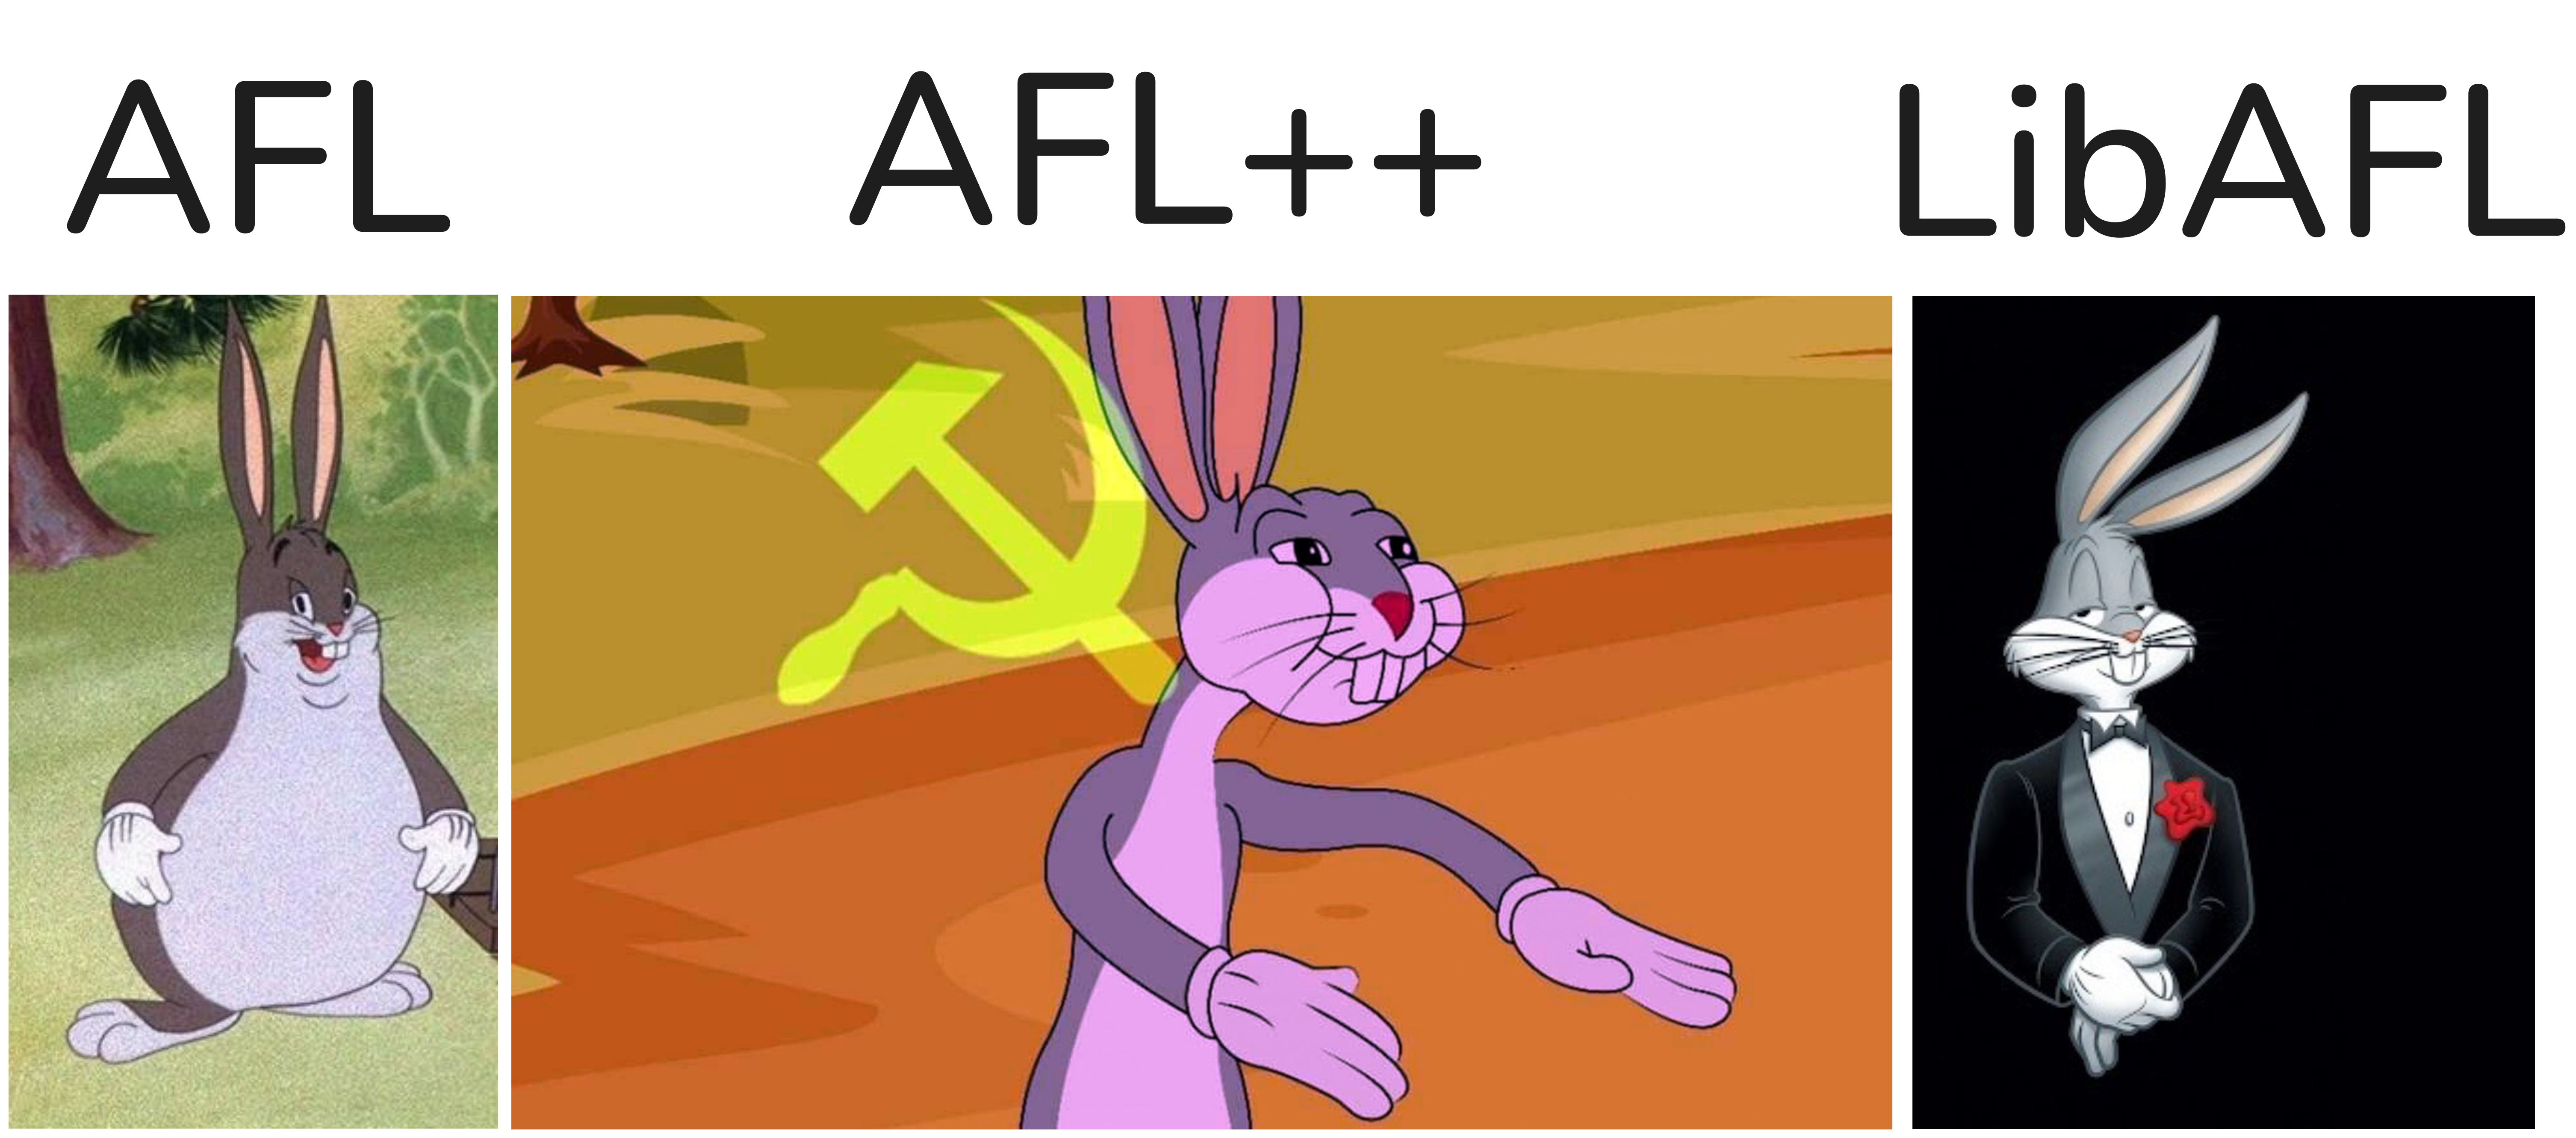
\includegraphics[width=0.95\textwidth]{assets/Afl_meme 2.png}
                \end{center}
        \end{figure}
\end{frame}

\begin{frame}{Why AFL?}
        \begin{itemize}
                \item Well documented and OSS
                \item Well maintained
                \item A lot of years of development $\rightarrow$ rock solid!
        \end{itemize}
\end{frame}

\begin{frame}{Why AFL?}
        \begin{itemize}
                \item (Runs only on *Nix and BSD like systems...)
        \end{itemize}
        \begin{figure}
                \begin{center}
                        \includegraphics[width=0.6\textwidth]{assets/Afl_meme 3.png}
                \end{center}
        \end{figure}
\end{frame}

\begin{frame}{AFL++}
        \begin{itemize}
                \item AFL with community patches - no need to fork you own copy of AFL and modify it!
                \item \textbf{Custom mutators API}: allow researchers to write their modification on top of AFL++ for
                        \begin{enumerate}
                                \item[a] (de)init
                                \item[b] input mutation
                                \item[c] trimming
                        \end{enumerate}
        \end{itemize}
\end{frame}

\begin{NoHyper}
\begin{frame}
        \section{DEMO}
        \sectionpage
\end{frame}
\end{NoHyper}

\begin{frame}{Demo}
        \begin{itemize}
                \item We will fuzz the \texttt{xpdf} and \texttt{libexif}, shoutout to Antonio Morales~\cite{morales} for his wonderful course!
                \item \textbf{Goals}
                        \begin{enumerate}
                                \item find \texttt{xpdf} bug and reproduce \href{https://www.cvedetails.com/cve/CVE-2019-13288/}{\texttt{CVE-2019-13288}}
                                \item reproduce \href{https://cve.mitre.org/cgi-bin/cvename.cgi?name=CVE-2012-2836}{\texttt{CVE-2012-2836}} for \texttt{libexif} using \texttt{exif} as frontend
                        \end{enumerate}
        \end{itemize}
\end{frame}

\begin{frame}{Hardware/software setup}
        \begin{itemize}
                \item \textbf{Hardware}
                        \begin{itemize}
                                \item 13th Gen Intel(R) Core(TM) i7-1355U
                                \item 32 GB RAM DDR4
                        \end{itemize}
                \item \textbf{Software}
                        \begin{itemize}
                                \item Debian 12
                                \item QEMU
                        \end{itemize}
        \end{itemize}
\end{frame}

\begin{frame}{Fixing \texttt{CVE-2019-13288}}
        \lstinputlisting{code/bug.cc}
        \lstinputlisting{code/solve.cc}
\end{frame}

\begin{frame}{Fixing \texttt{CVE-2012-2836}}
        \begin{enumerate}
                \item \href{https://github.com/libexif/libexif/commit/8ce72b7f81e61ef69b7ad5bdfeff1516c90fa361}{commit 8ce72b7f81e61ef69b7ad5bdfeff1516c90fa361}
                \item \href{https://github.com/libexif/libexif/commit/00986f6fa979fe810b46e376a462c581f9746e06}{commit 00986f6fa979fe810b46e376a462c581f9746e06}
        \end{enumerate}
\end{frame}

\begin{frame}{Conclusion}
        \begin{itemize}
                \item We had a (veery brief) overview about fuzzing
                \item We were able to successfully fuzz and reproduce real world CVEs on widely used open source software
                \item There is a lot of room for learning further =D
        \end{itemize}
\end{frame}

\begin{frame}{About this presentation...}
        It was entirely made with Open Source Software!
        \begin{itemize}
                \item[{\includegraphics[width=1em]{assets/aflpp}}] Aflplusplus fuzzer
                \item[{\includegraphics[width=1em]{assets/evince}}] Evince for sides presentation
                \item[{\includegraphics[width=1em]{assets/excalidraw}}] Excalidraw for diagrams (and memes)
                \item[{\includegraphics[width=1em]{assets/gimp}}] Gimp for memes only
                \item[{\includegraphics[width=1em]{assets/latex}}] \LaTeX/Beamer for slides
                \item[{\includegraphics[width=1em]{assets/neovim}}] Neovim for code
                \item[{\includegraphics[width=1em]{assets/qemu}}] QEMU for virtualization 
        \end{itemize}
\end{frame}

\begin{frame}[allowframebreaks]{Bibliography}
        \tiny
        \printbibliography
\end{frame}

\begin{NoHyper}
\begin{frame}{}
    \centering
        \begin{figure}
                \begin{center}
                        \includegraphics[width=0.6\textwidth]{assets/the_end.jpg}
                \end{center}
        \end{figure}
        
\end{frame}
\end{NoHyper}

\end{document}
